% kapitel3.tex
\chapter{ Collision Finding}
\label{chapter:kap3}
\section {About collisions }
Hash functions have resistance:
\begin{enumerate}
    \item First Preimage Resistance: for a hash function $h(m) = H$ the massage $m$ is hard to find.       
    \item Second Preimage Resistance: for a given messages $m_1$ it is hard to find an $m_2$ with $m_1 \neq m_2 $ and $h(m_1) = h(m_2)$.
    \item Collision Resistance: two arbitrary messages  $m_1$ and $m_2$ with $\neq m_2 $ and  $h(m_1) = h(m_2)$ are hard to find.
\end{enumerate}


\section{Differential Path}
Explain the genereal idea of the bit conditions first. There is a part I want to talk about the diffeces of Wang and Steven. In this part I can tear the details of the differential paths apart.


Stevens starts with Wang's attack, which tries to find to pairs of blocks:
\( \left(B_0 , B_0' \right) \)  and \( \left(B_1 , B_1' \right) \) that \( IHV = IHV' \),
 with the goal to create two massages $ M $ and $ M' $, with the same hash value:

\begin{align*}
    &IHV_0 &\xrightarrow[M_{(1)}] {}&\cdots &\xrightarrow[M_k]{} &IHV_k \xrightarrow[B_0]{} &IHV_{k + 1}  &\xrightarrow[B_1]{} &IHV_{k + 2}  &\xrightarrow[M_{k+1}]{}&\cdots &\xrightarrow[M_N]{} &IHV_N\\
    &=     &                        &       &                    &=                         &\ne          &                    &=            &                       &       &                    &= \\
    &IHV_0 &\xrightarrow[M_{(1)}] {}&\cdots &\xrightarrow[M_k]{} &IHV_k \xrightarrow[B_0]{} &IHV'_{k + 1} &\xrightarrow[B_1]{} &IHV'_{k + 2} &\xrightarrow[M_{k+1}]{}&\cdots &\xrightarrow[M_N]{} &IHV_N\\
\end{align*} 
The idea to manipulate a block $B$ such that $Q_1 \dots Q_{16}$ maintain their conditions and that $Q_17$ to some $Q_k$ do not change at all. We try to make k as large as possible.
\section{Bit Conditions}

Again, try to keep it theoretical, give an overview what we want to do with the bit conditions and safe the details for the comparison between Steven and Wang.



Bit conditions describe the differential path on bits. 
We need the bit conditions to avoid a carry, so a manipulation in step $t$ stays in step $t$ and does not propagate beyond the $31$st bit.
We look at conditions and restrictions. The restrictions leads to conditions, which we calculate in the following.
A restriction e.g. $\Delta T_2 \left[\ 31 \right] = +1 $ leads to conditions $ Q_1\left[ 16 \right] Q_2\left[ 16 \right] = Q_3\left[ 15 \right] = 0 $ and $ Q_2[15] = 1$.
Notice, conditions are on $\Delta T_t[i]$ a state in md5-algorithm before the rotation and restrictions are on $Q_t[i]$ states of the md5-algorithm after the rotation.\\ 
We calculate the bit conditions by using the Add-Difference for two massage blocks containing tow blocks $N|M$ and $N'|M'$. The XOR-Difference is useful, too.
    \begin{align*}
        \delta X &= X' - X \left( mod32 \right) \text{ Add-Difference}\\
        \Delta X &= X' \oplus X \text{ XOR-Difference}\\
        \lambda \left[i\right] &= \text{ our guess for the ith bit: } X\left[i\right] \\
        \\
        \text{if } \Delta X = \lambda &\Rightarrow \delta x \text{ can be determined}
    \end{align*}

For $\lambda \left[i\right]$ we only need to consider $i < 31$, since $X \left[ 31 \right]$ as msb always creates a add difference of $2^{31}$.\\
\begin{figure}
    \begin{align*}
        \delta F_t &= f \left( Q'_t,Q'_{t-1},Q'_{t-2} \right) \\
        \delta T_t &= \delta F_t + \delta  Q'_{t-3} + \delta W_t \\
        \delta R_t &=  RL \left(T'_t,RC_t \right) - RL \left(T_t,RC_t \right)\\
        \delta Q_{t+1} &= \delta Q_t + \delta R_t
    \end{align*}
    \caption[short]{Add difference}
    \label{md5delta}
\end{figure}
\newpage
\begin{wrapfigure}[]{r}{0.3\textwidth}
    %\begin{table}[]
        \begin{tabular}{| c | c | c |}
            \hline
            $t$ & $RC(t)$ & $AC(t)$    \\
            \hline
            \hline
            0  & 7  & \\
            1  & 12 & \\
            2  & 17 & \\
            3  & 22 & \\
            4  & 7  & \\
            5  & 12 & \\
            6  & 17 & \\
            7  & 22 & \\
            8  & 7  & \\
            9  & 12 & \\
            10 & 17 & \\
            11 & 22 & \\
            12 & 7  & \\
            13 & 12 & \\
            14 & 17 & \\
            15 & 22 & \\
            \hline
        \end{tabular}
        \caption{Overview of each rounds constants}
        \label{RC}

    %\end{table}
    \end{wrapfigure}
We calculate a $\delta$ for each $f_t$, $Q_t$, $T_t$ and $R_t$ for our add difference, to calculate $Q_{t+1}$ .
Additional we need the rotation constant $RC$ for each $t$. 
In general we begin with the $f_t$ since we want $f_t$ to be in a particular state.
Since we want to avoid a carries in our calculation 


\begin{enumerate}
    \item $t \in \{0,1,2,3\}$:\\
     $Q_t = 0 $ since here is no influence by an message and no calculation of f, there is nothing to change:
    \item $t = 4$\\
    $\Delta T_4 = -2^{31}$, because we must not have a carry, we \textit{lock} the last bit.
    Since  $RL(T_4, RC_4) = RL(-2^{31}, 7) = -2^6 $ and $\delta Q_4 = 0 \Rightarrow  \delta Q_5 = -2^6$  
\end{enumerate}
for an example we can use the detailed calculations of Wang's or maybe used our own, for a first understanding Wang's might be better.
Again, explain the bit conditions and not the differences between Steven's and Wang's Code.

\vfill
input 
\newpage

\section{Second Preimage Resistance}
Wang's attack of the MD5 bases on two algorithms. One processes the first and the other the second block of an arbitrary massage, without loss of generality (w.l.o.g.). We call it first block.
The first algorithm finds to the given first input block's IHV another IHV so that both blocks have the same new IHV.
Again it is important to notice that both blocks differ only a little form each other.     
In our approach we reconstructed the algorithm of Wang fitting our implementation of the \textit{MD5-Algorithm} and the code of Steven's attack.
We managed to provoke a second preimage resistance failure.  

\section{About Code}
There are multiple approaches to find the second block. Stevens used in his code five. Four written by himself.
They all have similarities, especially in the beginnings. 
The first \textit{find-first-block} algorithm though, is the algorithm by Wang. His additional algorithms are "just" improvements, if the algorithm of Wang does not success.
Since the similarities we only go in Wang's algorithm with a deeper view and explain some improvements eventually.\\
The question: "\textit{If there are "better" algorithms by Stevens, why start with Wang's anyway?}" may come up, yet we have to clarify what better could. The algorithm of Wang is quite efficient, but also in very minimalistic. 
The quote I have to check is, \textit{if the code by Wang finds a first block, it is in the most efficient way}, but it does not always find a first block were some is.
So using the algorithm by Wang as a first search algorithm, may increases our performance. It is also an more easy way to implement working code, since the algorithms of Stevens tend to be more complex, 
but also building up on Wang's.\\ 
The first 16 Qs can be chosen arbitrary, as long as we fulfill the conditions.
Stevens does this by generating really good random values.
After this he alters the random values so thy fulfill conditions.
We follow Stevens approach but generate "normal" random values and alter these so they fulfill the conditions
Improvements for random number generation are possible. \\
Example for Stevens bit manipulation for $Q_t$ with $t = 3$ :\\
\\
$1.$ the values to set the zeros (bitwise-and with $0xfe87bc3f$)\\
$2.$ the values to set the ones ( bitwise-or with $0x017841c0$)\\
$3.$ the new bit conditions\\
$4.$ the old bit conditions

\begin{align*}    
    1.& \text{ AND} & 11111110 & & 10000111 & & 10111100 & & 00111111 & & 0xfe87bc3f \\
    2.& \text{ OR}  & 00000001 & & 01111000 & & 01000001 & & 11000000 & & 0x017841c0 \\
    3.&             & ........ & & .1111... & & .1....01 & & 11...... & &  \\
    4.&             & ........ & & ....0... & & ....0... & & .0...... & &  
\end{align*}

  the $\&$ flips the $0$ correct, the $\|$ flips the $1$ correct\\
We now calculate the massage $m_t$ for $t \in \{0,6,\dots,15\} $. For this we use the reverse md5 function:
\begin{align*}
    m_t = RR \left( Q_{t+1} - Q_t , RC_t\right) - f_t \left( Q_t, Q_{t-1}, Q_{t-2} \right) - Q_{t-3} - AC(t)
\end{align*}
This function comes up by simply processing the MD5 sum \ref{md5sum} backwards.
We try to pick a $Q_{17}$ that $Q_{18}, \dots, Q_{21}$ can be calculated with $Q_{17},\dots,Q_{15}$ and fulfill their conditions. 
We can solve this by looping about the calculation as long as the conditions are not fulfilled and then brake. Note: we may calculate the values in temp variable before pasting them into the actual $Q$.\\
\begin{wrapfigure}[]{r}{0.4\textwidth}
    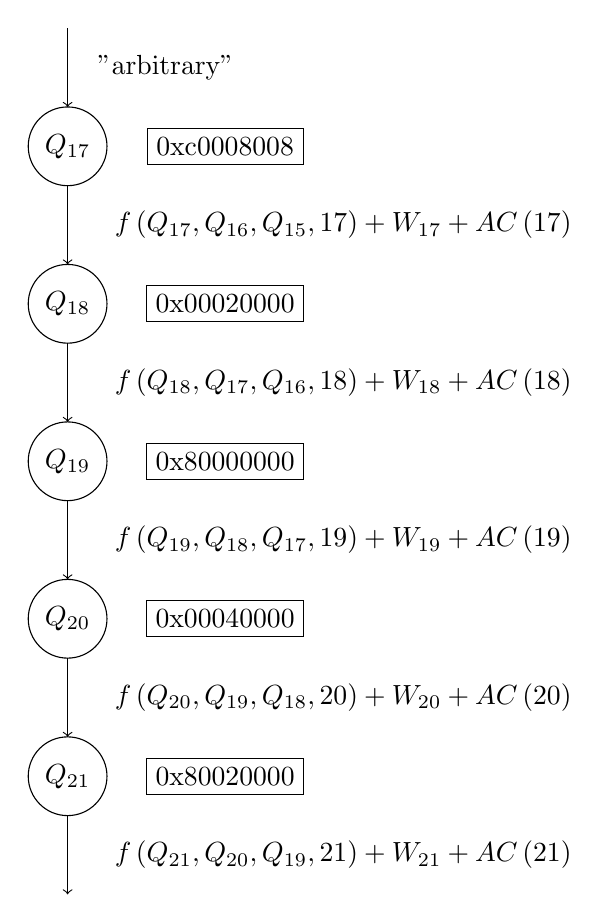
\begin{tikzpicture}
        \tikzstyle{every node}=[font=\normalsize]
        \draw  (6.75,24) circle (0.5cm) node{\normalsize $Q_{17}$};
        \draw  (6.75,22) circle (0.5cm) node{\normalsize $Q_{18}$};
        \draw  (6.75,20) circle (0.5cm) node{\normalsize $Q_{19}$};
        \draw  (6.75,18) circle (0.5cm) node{\normalsize $Q_{20}$};
        \draw  (6.75,16) circle (0.5cm) node{\normalsize $Q_{21}$};

        \draw [ -to] (6.75,25.5) -- (6.75,24.5) ;
        \draw [ -to] (6.75,23.5) -- (6.75,22.5);
        \draw [ -to] (6.75,21.5) -- (6.75,20.5);
        \draw [ -to] (6.75,19.5) -- (6.75,18.5);
        \draw [ -to] (6.75,17.5) -- (6.75,16.5);
        \draw [ -to] (6.75,15.5) -- (6.75,14.5);

        \node[] at (8,25) {\normalsize "arbitrary"};
        \node[] at (10.25,23) {\normalsize $f\left( Q_{17},Q_{16},Q_{15},17\right) + W_{17} + AC\left(17\right)$};
        \node[] at (10.25,21) {\normalsize $f\left( Q_{18},Q_{17},Q_{16},18\right) + W_{18} + AC\left(18\right)$};
        \node[] at (10.25,19) {\normalsize $f\left( Q_{19},Q_{18},Q_{17},19\right) + W_{19} + AC\left(19\right)$};
        \node[] at (10.25,17) {\normalsize $f\left( Q_{20},Q_{19},Q_{18},20\right) + W_{20} + AC\left(20\right)$};
        \node[] at (10.25,15) {\normalsize $f\left( Q_{21},Q_{20},Q_{19},21\right) + W_{21} + AC\left(21\right)$};
        
        \node[draw] at (8.75,24) {\normalsize 0xc0008008 };
        \node[draw] at (8.75,22) {\normalsize 0x00020000 };
        \node[draw] at (8.75,20) {\normalsize 0x80000000 };
        \node[draw] at (8.75,18) {\normalsize 0x00040000 };
        \node[draw] at (8.75,16) {\normalsize 0x80020000 };
        \end{tikzpicture}    
    \label{demepndeces}
\end{wrapfigure}
For a good pick for $Q_{17}$ we just generate a random value and force the conditions manual.
\newpage
6
